\chapter{Background}
\section{Interpretability}
\begin{itemize}
	\item Need for Interpretability
\end{itemize}
\section{Gradient Based Explanations}
\begin{itemize}
	\item Taxonomy
\end{itemize}
\section{Augmentation}
\begin{itemize}
	\item Taxonomy
\end{itemize}
\section{Datasets}
To test Proxy Attention, the following datasets were used.
Note: Images are resized to 224x224 pixels for consistency. These batch visualizations are generated by the author using the torchvision and matplotlib libraries.

\subsection{CIFAR 100}
The CIFAR 100 dataset, introduced by \cite{krizhevskyLearningMultipleLayers} is an image dataset with 60000 color images with dimensions 32x32 pixels. As the name suggests, the dataset has 100 unique classes. Each of these classes have 500 training images. Some of the classes are - airplane, bird, truck, ship, deer and dog. This dataset is used as a coarse grained classification dataset in this project.

\resizebox{.8\textwidth}{!}{

	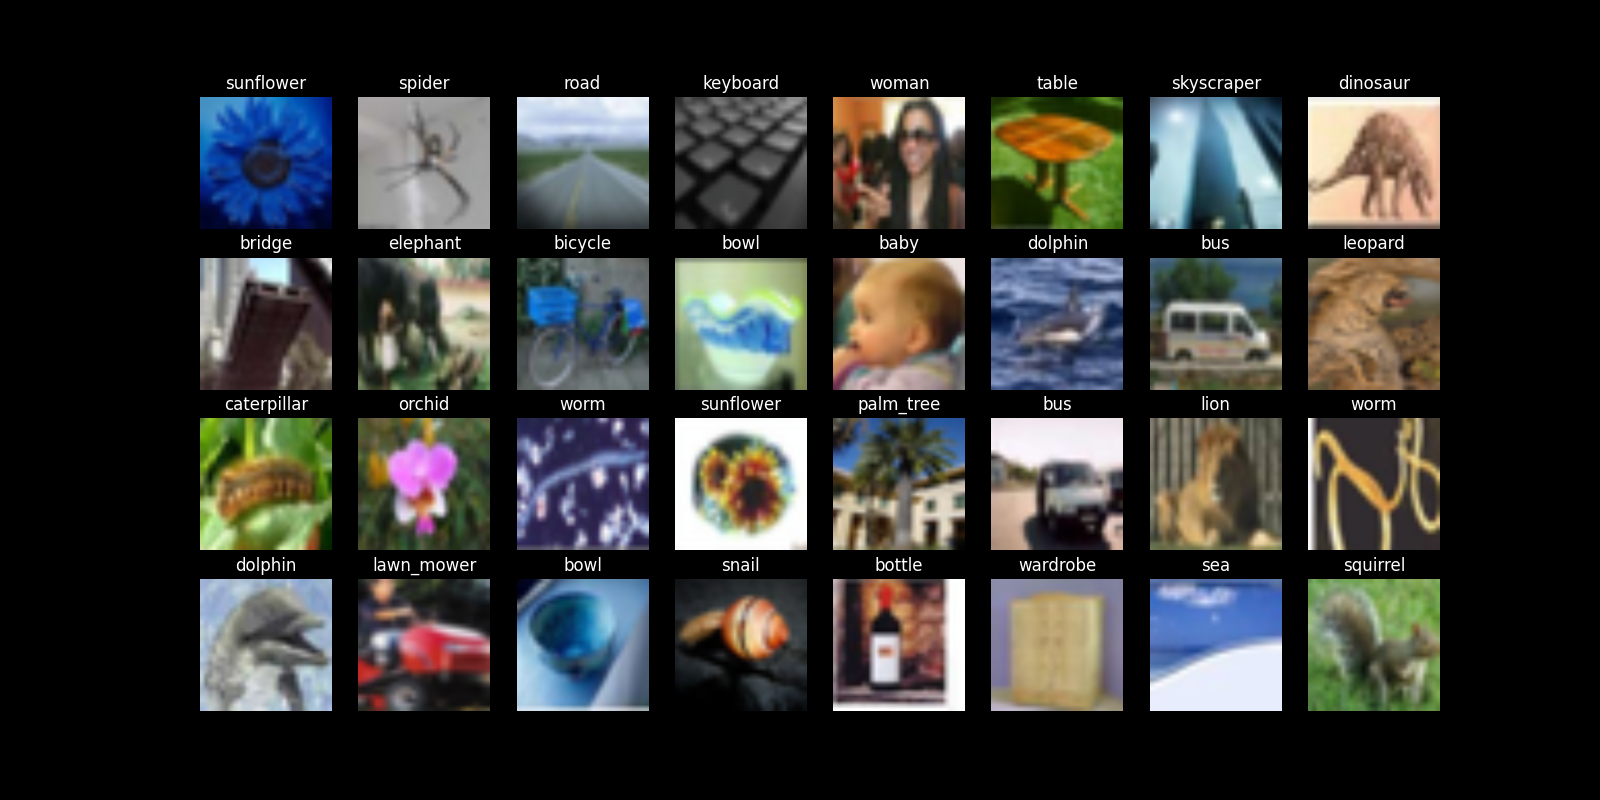
\includegraphics{images/cifar100.png}
}
% \subsection*{IIT pets}
% \resizebox{.8\textwidth}{!}{

% 	\includegraphics{images/iitpets.png}
% }
\subsection{Stanford dogs}

\resizebox{.8\textwidth}{!}{
	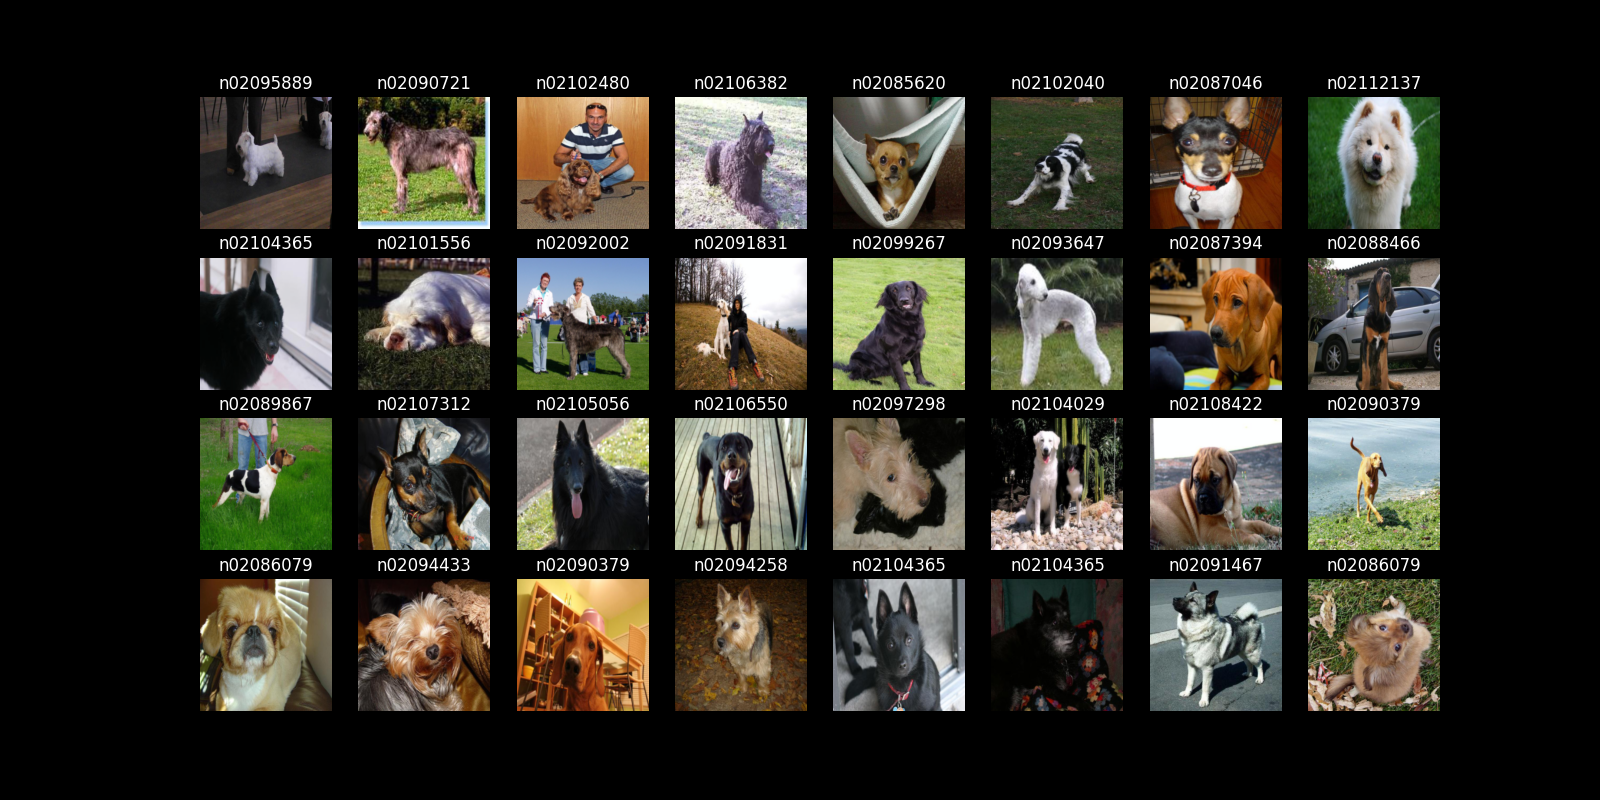
\includegraphics{images/dogs.png}
}
\subsection{Imagenette}
\resizebox{.8\textwidth}{!}{
	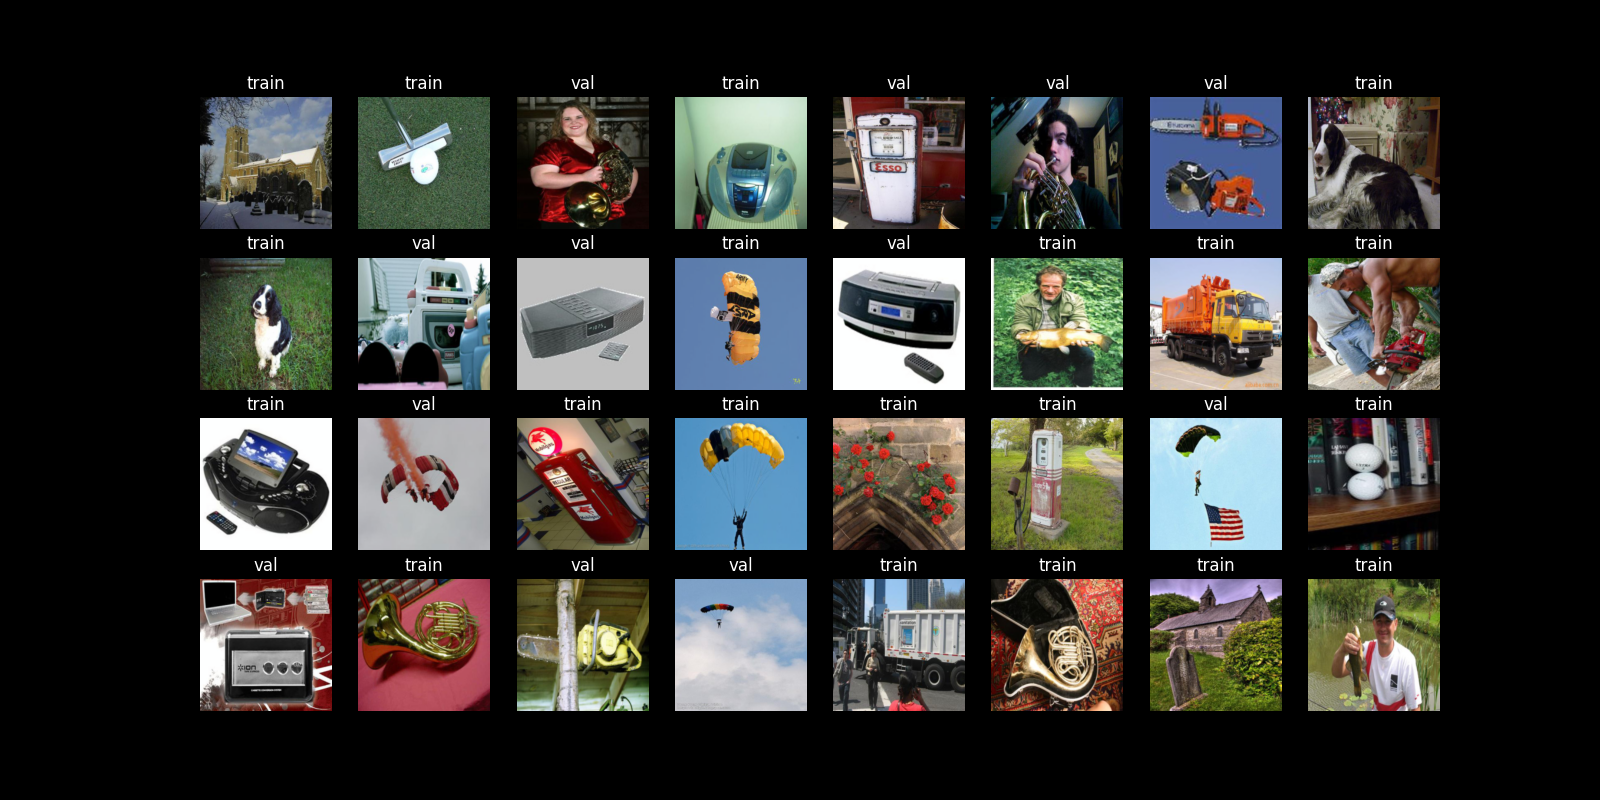
\includegraphics{images/imagenette.png}
}
\subsection{ASL}
\resizebox{.8\textwidth}{!}{
	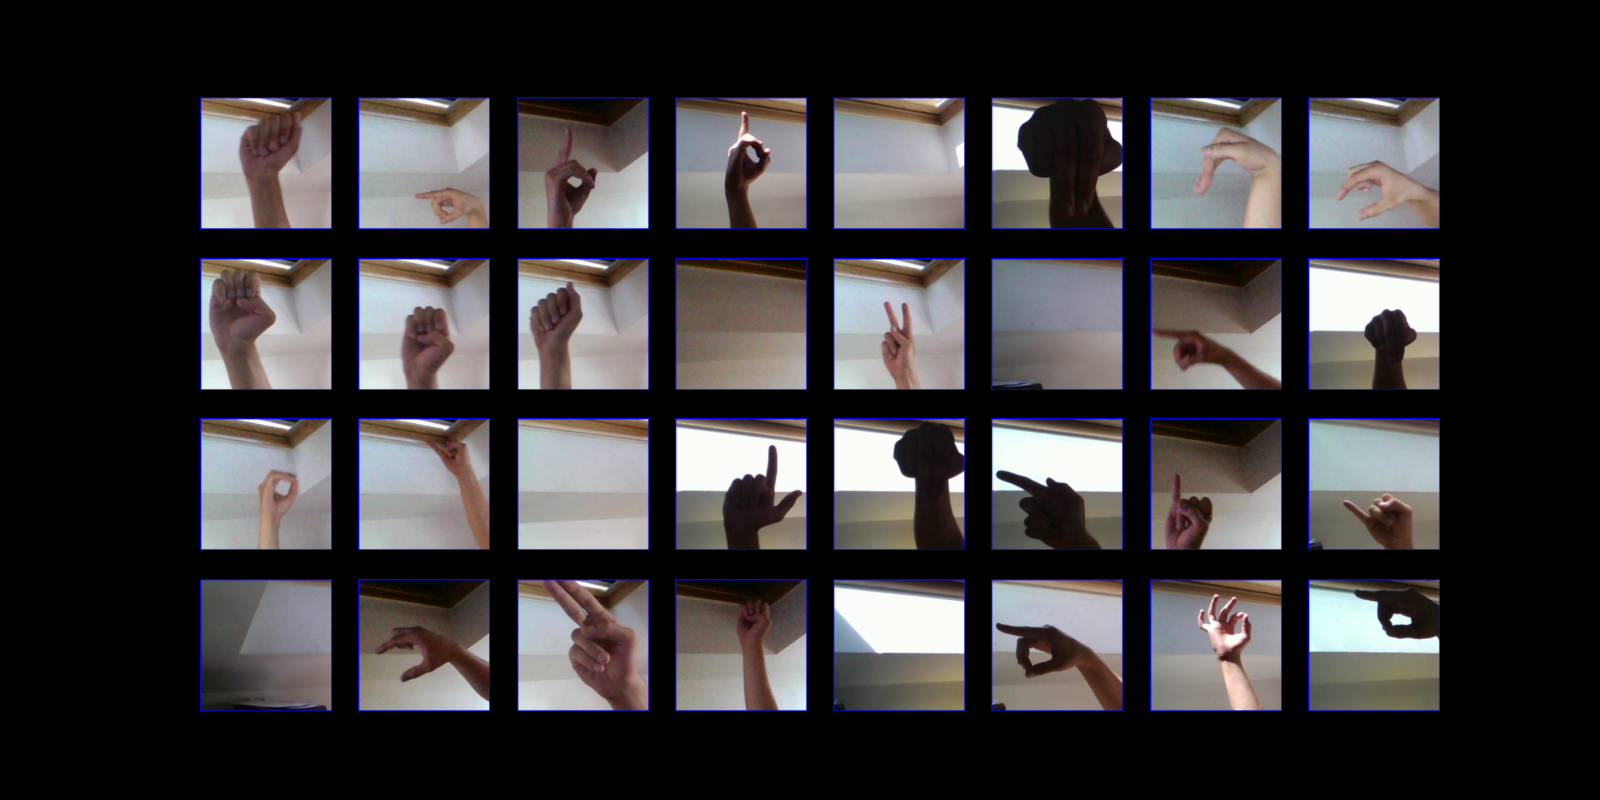
\includegraphics{images/asl.png}
}

\subsection{Food-101}

\subsection*{Plant Village}